\chapter{Konzeption und Methodik}\label{ch5}
In diesem Kapitel geht es darum, den Konzept des praktischen Teils der Arbeit wiederzugeben. Der praktische Teil der Arbeit besteht aus 3 Bereichen. Zunächst wird ein Datensatz erstellt, dann wird anhand der Daten aus diesem Datensatz ein Modell trainiert und schließlich wird dieses Modell in eine Webanwendung umgewandelt (siehe Abbildung~\ref{Kap5:Konzeption}). In diesem Abschnitt soll klargestellt werden, wie ein clientseitiges Deep Learning für deutsche Clickbaits stattfinden kann. Es wird also untersucht, welche Methoden angewendet werden können und es werden die ersten Vorüberlegungen vorgestellt, welche in den weiteren Kapiteln durch praktische Anwendung explizit werden.

\begin{figure}[H]
    \centering
    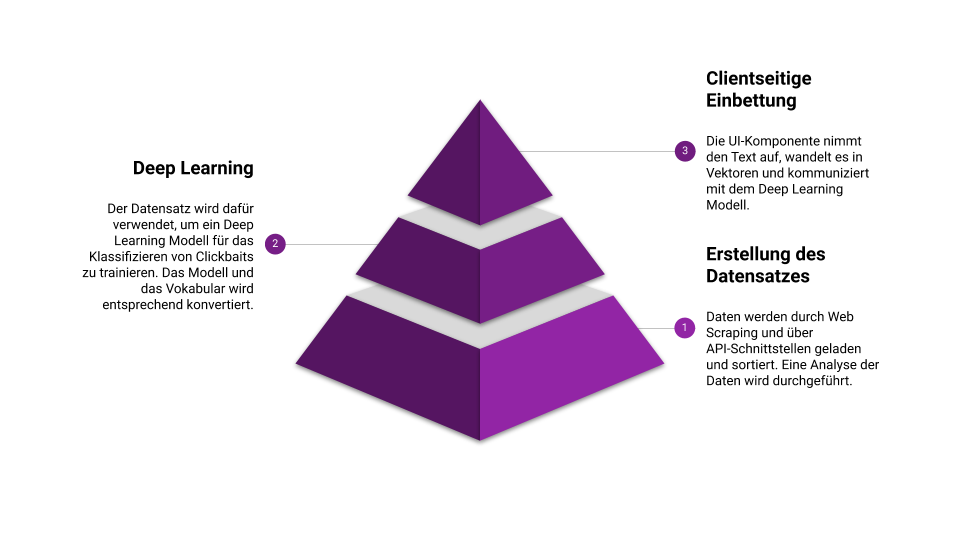
\includegraphics[width=15cm]{kapitel5/main_p.png}
    \caption[Darstellung der Konzeption]{Darstellung der Konzeption}
    \label{Kap5:Konzeption}
\end{figure}



Deep Learning Modelle benötigen eine große Menge an Beispielen um zu lernen. Neben der Anzahl an Daten, muss auch ein Zusammenhang zwischen den Daten und dem Modell herrschen. In der Arbeit von von \cite*{Chakrabortya}, haben die Autoren Daten aus dem Web geladen. Sie sind dabei so vorgegangen, dass sie bestimmte Seiten gecrawlt haben, die viele Clickbaits beinhalten und als Kontrast zu diesen Nachrichten Wikinews herangezogen haben. Ähnlich kann also vorgegangen werden. Es müssen zunächst einige Seiten gefunden werden, die deutsche Clickbaits oder \enquote{Unterhaltungsnachrichten} mit ähnlichen Charakter wie Clickbaits gefunden werden. Wikinews bietet auch eine deutsche Version. Wikipedia bietet eine offene API, welches auch für die Nachrichten benutzt werden kann. Diese API kann dafür verwendet werden, um deutsche Nachrichtentitel zu extrahieren. Die Wikipedia-News-API bietet einen Kostenlosen Endpunkt an, welches verschiedene Nachrichtenportale wie z.B. Politik, Wirtschaft, Kultur, Sport und Wissenschaft anbietet.  Die Datenaquise für Clickbaits verläuft dagegen anders. Der Datensatz von \cite*{Chakrabortya} beinhaltet jeweils 7.500 Nachrcihten je Kategorie. Es ist zu berücksichtigen, dass diese Studie nicht mit Deep Learning Modellen arbeiten, sondern mit klassischen Machine Learning Algorithmen. Um die Datenextraktion zu automatisieren bietet sich die Software \textit{Scrapy} an. Scrapy ist ein Open-Source Tool, welches das extrahieren von großen Mengen an Daten erleichtert. Es ist in Python geschrieben und kann durch seine Middleware Funktion erweitert werden. Die Daten können so z.B. direkt in eine SQL-Datenbank geschrieben werden.


Der mittlere Kern der Pyramide in Abbildung~\ref{Kap5:Konzeption} ist das Deep Learning Modell, welches als Inferenzmaschine betrachtet werden. Es wird durch die Eingabe der gekennzeichneten Daten trainiert und in ein entsprechendes Format gebracht. Es gibt mehrere Anbieter für das Deep Learning. Die meisten von Ihnen sind Open Source. Die bekanntesten Bibliotheken für das Deep Learning sind \textit{TensorFlow} (welches von Google unterstützt wird) und PyTorch (welches von Facebook unterstützt wird). Seit März 2018 bietet TensorFlow die Möglichkeit, Modelle in der Programmiersprache JavaScript zu trainieren und zu benutzen. Klassischerweise werden Deep Learning Modelle dem Endbenutzer durch das Web angeboten. Es wird zunächst ein Modell trainiert und dann auf einem Server geladen. Der Server bietet einen HTTP-Endpunkt an, welches die Schnittstelle zwischen dem Nutzer und des Modells ist. Durch \textit{TensorFlow.js} wird das Modell in den Speicher des Nutzers, also in seinen Browser geladen. Dann kann der Nutzer mit diesem Modell im Speicher wesentlich einfacher kommunizieren. Um dieses zu verwirklichen sind aber bestimmte Voraussetzungen nötig. Erstens muss dass Modell in irgendeiner Art und Weise in einer Form sein, welches eine solche Benutzung zulässt. Zweitens muss das Modell die Eingabe des Nutzers verstehen. Drittens muss das Modell in die Umgebung eingebaut werden. Das Modell kann auch komplett auf TensorFlow.js trainiert werden. TensorFlow.js läuft in JavaScript, kommuniziert aber mit der TensorFlow-API. Es bieten sich zwei Möglichkeiten des Trainings an. Entweder kann das Modell in JavaScript mit TensorFlow.js trainiert werden oder das Modell wird herkömmlich mit TensorFlow trainiert und dann durch eine Konvertierung in ein Format gebracht, welches in TensorFlow.js laufen kann. 

Das Ergebnis der Arbeit ist die Einbettung des Modells in eine Benuteroberfläche. Es sollte eine Benuteroberfläche entstehen, welches die Eingabe des Nutzers versteht und in einer Art und Weise dem Modell, welches in den Browser geladen werden muss, weitergibt. Das Modell muss mit der UI kommunizieren. Das Frontend wird in JavaScript geschrieben. Im modernen JavaScript gibt es UI-Bibliotheken die das Frontend flexibler und einfacher gestalten lassen als nur mit JavaScript alleine. Es wird die Bibliothek \textit{React} verwendet, um den Zusammenhang zwischen Deep Learning und moderner Webentwicklung zu verwirklichen.

